Deep Convolutional Neural Networks have become the \emph{de facto} solution for
image understanding tasks since the rapid development in their growth in recent
years. Since AlexNet\autoref{krizhevsky_imagenet_2012} in 2012, there have been
many new improvements in their design, taking them `deeper', such as the
VGG network in 2014 \cite{simonyan_very_2014}, the Inception Network
\cite{szegedy_going_2015}, Residual Networks in 2016
\cite{he_deep_2016} and DenseNets in \cite{huang_densely_2017}. Each iteration
has made the inner workings of the model more and more abstract.

Despite their success, Deep Nets are often criticized for being `black box'
methods. Indeed, once you train a CNN, you can view the first layer of filters
quite easily (see \autoref{fig:alexnet_filters}) as they exist in RGB
space. Beyond that things get trickier, as the filters have a third, `depth'
dimension typically much larger than its two spatial dimensions, and
representing these dimensions with different colours becomes tricky and
uninformative.

This has started to become a problem, and while we are happy to trust modern
CNNs for isolated tasks, we are less likely to be comfortable with them driving
cars through crowded cities, or making executive decisions that affect people
directly. In a commonly used contrived example, it is not hard to imagine a deep
network that could be used to assess whether giving a bank loan to an applicant
is a safe investment. Trusting a black box solution is deeply unsatisfactory in
this situation. Not only from the customer's perspective, who, if declined, has
the right to know why \cite{goodman_european_2016}, but
also from the bank's --- before lending large sums of money, most banks
would like to know why the network has given the all clear. `It has worked well
before' is a poor rule to live by.

A recent paper titled `Why Should I Trust You?' \cite{ribeiro_why_2016}
explored this concept in depth. They rated how highly humans trusted machine
learning models. Unsurprisingly, a model with an interpretable methodology
was trusted more than those which did not have one, even if it had a lower
prediction accuracy on the test set. 
To build trust and to aid training, we need to probe these networks and
visualize how and why they are making decisions.
% One of their measures of
% `interpretability' for image classifiers involved finding the regions of the
% input image that caused a high output for that particular class --- see
% \autoref{fig:ch4:interpretability}. 

Some good work has been done in this area. In particular,
Zeiler and Fergus \cite{zeiler_visualizing_2014} 
design a DeConvNet to visualize what input patterns a filter in a given layer is mostly highly
activated by. In \cite{mahendran_understanding_2015},
\citeauthor{mahendran_understanding_2015} learn to invert
representations by updating a noisy input until its latent feature vector
matches a desired target. \cite{simonyan_deep_2014} develop saliency maps by
projecting gradients back to the input space and measuring where they have
largest magnitude.

In recent years, ScatterNets have been shown to perform well as image
classifiers and have received a fair share of attention themselves. They have
been one of the main successes in applying wavelets to
deep learning systems, and are particularly inspiring due to their well defined
properties.  They are typically used as unsupervised feature extractors
\cite{bruna_invariant_2013, oyallon_deep_2015, 
singh_dual-tree_2017, singh_multi-resolution_2016} and 
can outperform CNNs for classification tasks with reduced
training set sizes, e.g.\ in CIFAR-10 and CIFAR-100 (Table 6 from
\cite{oyallon_scaling_2017} and Table 4 from \cite{singh_dual-tree_2017}).  
They are also near state-of-the-art for Texture Discrimination tasks
(Tables 1--3 from \cite{sifre_rotation_2013}). Despite this, there still exists
a considerable gap between Scatternets and CNNs on challenges like CIFAR-10 with the
full training set ($~83\%$ vs.\ $~93\%$). Even considering the benefits of
ScatterNets, this gap must be addressed.

While ScatterNets have good theoretical foundation and properties
\cite{mallat_group_2012}, it is difficult to understand the second order
scattering. In particular, how useful are the second order coefficients for
training? How similar are the scattered features to a modern state of the art
convolutional network? To answer these questions, this chapter interrogates
ScatterNet frontends. Taking inspiration from the interrogative work applied to
CNNs, we build a DeScatterNet to visualize what the second order features are.
We also heuristically probe a trained Hybrid Network and quantify the importance
of the individual features.

We first define the operations that form a ScatterNet in
\autoref{sec:ch4:scatternet}. We then introduce our DeScatterNet
(\autoref{sec:ch4:descatternet}), and show how we can use it to examine the
layers of ScatterNets (using a similar technique to the CNN visualization in
\cite{zeiler_visualizing_2014}). We use this analysis tool to highlight what
patterns a ScatterNet is sensitive to (\autoref{sec:ch4:visualization}), showing
that they are very different from what their CNN counterparts are sensitive to,
and possibly less useful for discriminative tasks. 

We then measure the ScatterNet channel saliency by peforming an occlusion test
on a trained hybrid network ScatterNet-CNN, iteratively switching off individual
Scattering channels and measuring the effect this has on the validation accuracy
in \autoref{sec:ch4:occlusion}. The results from the occlusion tests strengthen
the idea that some of the ScatterNet patterns may not be well suited for deep 
learning systems.

We use these observations to propose an architectural change to ScatterNets,
which have not changed much since their inception in \cite{mallat_group_2012}, 
and show that it is possible to get visually more appealing shapes by filtering
across the orientations of the ScatterNet. We present this in
\autoref{sec:ch4:corners}.

% One of the key benefits of CNNs is their ability to take raw images and learn
% features --- i.e.,\ they do not require you to construct feature vectors. The
% paradigm that they are built on is really quite elegant --- you set up
% a network, you feed in your images, you define a cost function, and then you
% propagate error gradients to learn your representation. Unfortunately, the process
% rarely goes so smoothly. There are entire sets of hyperparameters that must
% be searched to find optimal solutions. Some hyperparameters (such as learning
% rate and initialization weights), can be so sensitive as to cause
% the network to diverge if they are set outside of a small range. Others, such
% as network depth and width often have counter-intuitive effects on the
% result. A commonly known one is that increasing the depth of a network often
% causes the accuracy to decrease, even though it should at worst remain
% constant, as the network could learn the identity mapping for deeper layers.

% Considering the recent success of CNNs, it is becoming more and more
% important to understand \emph{how} and \emph{what} a network learns, which
% has contributed to it making its classification or regression choice.
% Without this information, the use of these incredibly powerful tools could be
% restricted to research and proprietary applications.


  % \begin{figure}
    % \centering
      % 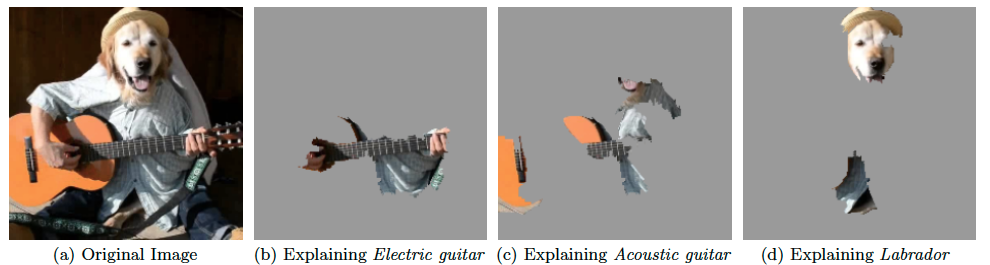
\includegraphics[width=\textwidth]{\imgpath/interpretability}
      % \mycaption{Explaining an image classification prediction made by Google's
      % Inception neural network}{The top 3 classes predicted are `Electric Guitar'
      % (p=0.32), `Acoustic Guitar' (p=0.24) and `Labrador' (p=0.21). The
      % regions which contributed to these predictions are shown in (b) through
      % (d)}
      % \label{fig:ch4:interpretability}
  % \end{figure}

% In image understanding tasks such as classification, recognition, and segmentation,
% Convolutional Neural Networks (CNNs) have now become the  and the state
% of the art model. Since they proved their worth in 2012 by winning the ImageNet
% Large Scale Visual Recognition Competition (ILSVRC) \cite{russakovsky_imagenet_2014}
% with the AlexNetwork \cite{krizhevsky_imagenet_2012}, they have been fine-tuned and developed into very
% powerful and flexible models. Most of this development has been in changing the
% architecture, such as the Residual Network\cite{he_deep_2016}, the Inception
% Network \cite{szegedy_going_2015} and the DenseNet \cite{huang_densely_2017}.
% However one of the key building blocks of CNNs, the convolutional filter bank,
% has seen less development and in today's models, they are not too dissimilar to
% what they were in 2012. % 


% In this chapter, let us look at similar techniques, i.e. zeiler.

% Then look propose the descattering

% then look at performance of newtorks when channels are turned off.

% Not sure how to do the corners work?



